\documentclass[main.tex]{subfiles}
\begin{document}

\section*{Mon Nov 18 2019}

\paragraph{Optically thick line}

In this case, the assumption is that \(\tau_{\nu } \gg 1\): all the radiation which is at the appropriate frequency will get absorbed.

The absorption in a unit volume will be proportional to the difference in velocities at its edges, which is then proportional to the gradient of the velocity.

The formula we then get is 
%
\begin{align}
g _{\text{line}} = \frac{F_{\nu }}{c} \frac{\nu_0}{c}
\frac{1}{\rho } \dv{v}{r} 
\propto \frac{L_{\nu }}{r^2} \frac{1}{\rho } \dv{v}{r}
\,,
\end{align}
%
so we have the same dependence as before with an additional factor.

\paragraph{Line pressure estimates}

% Let us come back to 
% %
% \begin{align}
%   g_l = \frac{F_\nu }{c} \frac{n_i}{\rho } \frac{\pi e^2}{m_e c} f \sim \frac{L_{\nu }}{r^2} \frac{n_i}{\rho }
% \,.
% \end{align}

We can reduce drastically the number of spectral lines we have to account for if we assume that, since the density of the wind is very low, collisional excitation is negligible: only lines from the ground state, low energy states and metastable states have to be accounted for. 
Even with this consideration, the number of lines to consider is still in the hundreds of thousands. 

We need to sum over all the optically thick and thin lines and everything in between.

% How do we deal with the radiation pressure for an ensemble of lines?
In order to do this, Castor, Abbott and Klein (CAK)
showed in 1975 that a reasonable estimate is:
%
\begin{align} \label{eq:general-line-velocity-gradient-dependence}
  g_{L} \sim \qty(\rho^{-1} \dv{v}{r})^{\alpha }
  \sim \qty(\frac{vr^2}{\dot{M}} \dv{v}{r})^{\alpha }
\,, \marginnote{From the continuity equation \(\dot{M} \propto r^2 \rho v\).}
\end{align}
%
where \(\alpha \) is a parameter quantifying the optical thickness of the line: it goes from \(0\) for an optically thin line to \(1\) for an optically thick line. 
% In general we have , which justifies the expression here.

The expression proposed by CAK was \(g_L = g_e M(t)\), where \(g_e\) is the radiative acceleration from continuum phenomena (mostly electron scattering), while the \emph{force multiplier} \(M\) is in the form: 
%
\begin{align}
  M(t)  = k t^{-\alpha } s^{ \delta }
\,,
\end{align}
%
where \(k , \alpha , \delta \) are called \emph{force multiplier parameters}. The variables \(t\) and \(s\) will be defined shortly.

The radiative acceleration due to electron scattering is given by 
\todo[inline]{Maybe we could keep a consistent notation between things? Why write first \(g_e\) and then \(g_L (e)\)? Frustrating.}
%
\begin{align}
  g_e = \frac{\kappa _e}{c} \frac{L_{*}}{4 \pi r^2} = \Gamma _e \frac{GM_{*}}{r^2}
\,,
\end{align}
%
where \(\Gamma _e \) is the so-called \emph{Eddington factor}: 
%
\begin{align}
  \Gamma _e = \frac{\kappa _e}{4 \pi c G} \frac{L_{*}}{M_{*}}
\,,
\end{align}
%
which is the luminosity divided by the Eddington luminosity.

The scattering opacity \(\kappa _e\) is given by 
%
\begin{align}
  \kappa _e \approx \frac{\sigma_{e}}{m_H }
\,,
\end{align}
%
which is measured in \SI{}{cm^2g^{-1}}. The value \(\sigma _e = \SI{6.65e-25}{cm^2}\) is the Thomson scattering cross section for electrons. This ratio gives \SI{0.39}{cm^2/g}, the value used by CAK is \SI{.325}{cm^2/g}, which is of the same order of magnitude and probably accounts for some other effects.

The \(t\) in \(M(t)\) is defined by 
%
\begin{align}
  t \equiv \kappa _e v _{\text{thermal}} \rho \dv{r}{v}
  = \kappa_e \sqrt{\frac{2 k_B T}{m_H}} \rho \dv{r}{v}
  = \kappa_{e} \sqrt{\frac{2 k_B T}{m_H}} \qty(\frac{1}{\rho } \dv{v}{r})^{-1}
\,,
\end{align}
%
and is inversely proportional to the velocity gradient divided by the density: so, since it is elevated to the \(- \alpha \), it gives the same contribution as the term in \eqref{eq:general-line-velocity-gradient-dependence}.

The \(s\) in the definition of \(M(t)\) contains information about the degree of ionization: it is 
%
\begin{align}
  s \equiv \frac{\num{e-11} \rho }{m_H W}
\,,
\end{align}
%
where \(W\) is the \emph{geometrical dilution factor}: 
%
\begin{align}
  W(r) = \frac{1}{2} \qty(1 - \sqrt{1 - \qty(\frac{R_{*}}{r})^2})
  \sim \qty(\frac{R_{*}}{2r})^2
\,,
\end{align}
%
and now we present a proof for the fact that this encodes the radial dependence of the observed intensity. 
It is a ratio of solid angles: 
%
\begin{align}
  W(r) = \frac{\int _{0}^{\Omega } \dd{\Omega } }{4 \pi }
\,,
\end{align}
%
where the integration limit \(\Omega \) encodes the solid angle subtended by the star.
Assuming simmetry with respect to the azimuthal angle, we can rewrite it as: 
%
\begin{align}
  W (r) = \frac{2 \pi }{4 \pi } \int _{0}^{\theta_1 } \sin \theta  \dd{\theta } 
  = \frac{1}{2} \int _1^{\cos(\theta_1 )} (-\dd{x}) 
  = \frac{1}{2} \qty(1 - \sqrt{1 - (R/r)^2})
\,,
\end{align}
%
so \(W(r)\) is the solid angle fraction subtended by a star with radius \(R\) at a distance \(r\). 

The complete expression for an ensemble of lines is given by 
%
\begin{align}
  g_L = \frac{\kappa _e}{ c} \frac{L_{*}}{4 \pi r^2} k t^{- \alpha } s^{ \delta }
\,,
\end{align}
%

Simulations show that \(M(t)\) decreases with \(t\) with some kind of power law: the approximation \(\log M \sim - \alpha \log t\) is justified. 

Numerical simulations show that \(\alpha \sim 0.5 \divisionsymbol 0.6\), independent of temperature.
The \(\delta\) parameter is almost always of the order \(\delta \sim 0.1\).

The force multiplier is also linearly dependent on the metallicity of the star: \(M_n(t_n) = M_n (t_n)_{\odot} (Z/Z_{\odot})\).

A typical velocity gradient is something like 
%
\begin{align}
  v(r) = v_{ \infty } \qty(1 - \frac{r_0 }{r})^{\beta }
\,,
\end{align}
%
with \(\beta \sim 0.7\).
Then, the profile of \(g_L\) can be computed (using the continuity equation): it is in the form 
%
\begin{align}
  g_L \sim r^{-2} \qty(\rho \dv{r}{v})^{-\alpha }
  \sim r^{2(\alpha -1)} \qty(v \dv{v}{r})^{\alpha }
\,, \marginnote{\(r^2 v \rho = \const\) by continuity}
\end{align}
%
where \(\alpha \sim 0.6\). The \(r\) dependence is something like 
%
\begin{align}
  g_L \sim r^{-2} \qty(1 - \frac{r_0 }{r})^{\alpha (2 \beta -1)}
\,,
\end{align}
%
which we can plot. 

\begin{figure}[H]
\centering
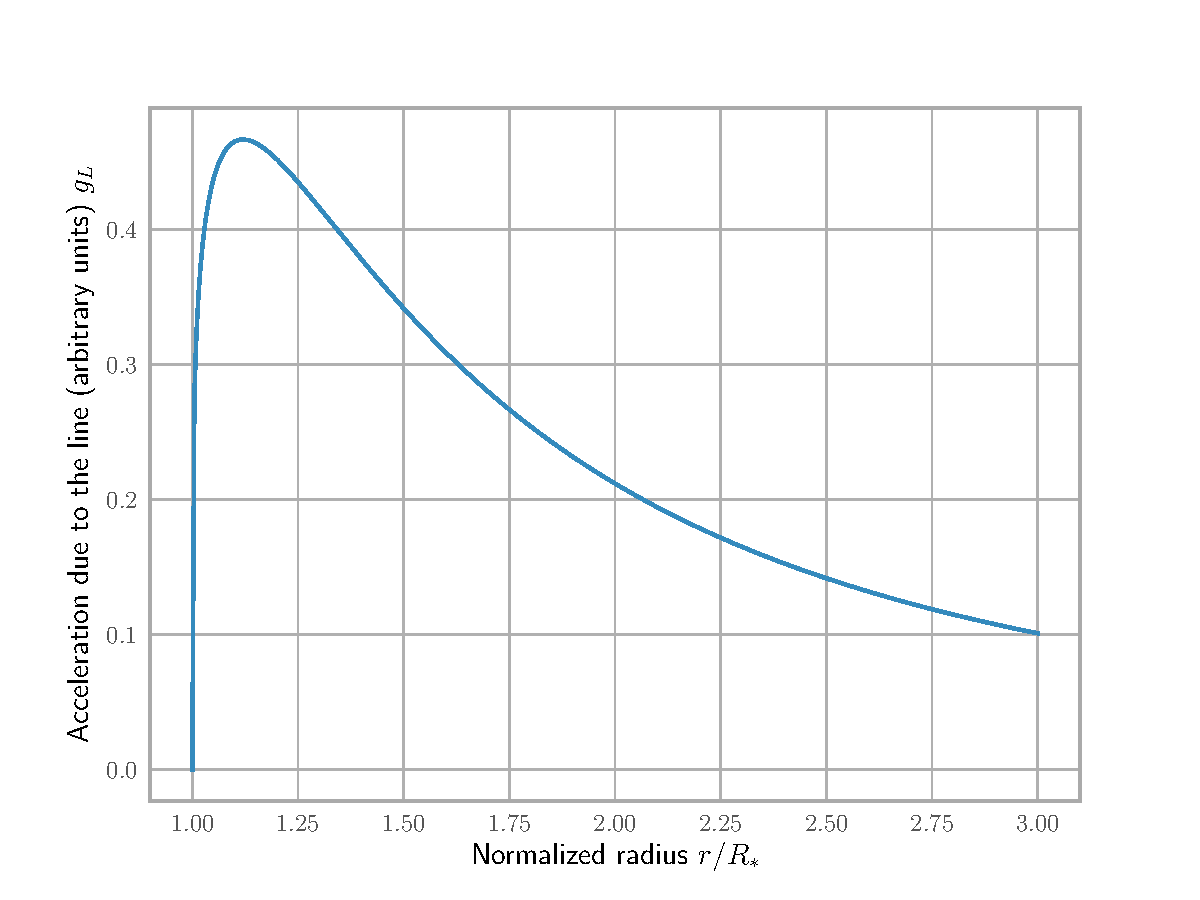
\includegraphics[width=\textwidth]{figures/line_acceleration_profile.pdf}
\caption{Line acceleration profile for \(\alpha = \num{.6}\) and \(\beta = \num{.7}\).}
\label{fig:line_acceleration_profile}
\end{figure}

\end{document}